\documentclass{beamer}
\usetheme{Warsaw}

\usepackage{polski}
\usepackage{graphicx}

\title{Principal Component Analysis (PCA)}
\subtitle{Redukcja Wymiarów i Ekstrakcja Cech}
\author{Piotr Kędzierski \& Mariusz Godlewski}
\date{}



\begin{document}
	
	
	\begin{frame}
		\titlepage
	\end{frame}
	
	
	\begin{frame}{Czym jest PCA?}
		\textbf{Principal Component Analysis (PCA)} jest metodą nienadzorowanego uczenia maszynowego używaną do upraszczania z skomplikowanych zbiorów danych.
		
		\vspace{0.5cm}
		\begin{itemize}
			\item \textbf{Redukcja Wymiarów:} PCA zmniejsza ilość zmiennych (wymiarów) używanych do opisu 
			\item \textbf{Zachowanie Informacji:} Stara się zachować jak najwięcej wariancji (w domyśle ważnych cech) przy jak najmniejszej ilości komponentów.
			\item \textbf{Usunięcie Korelacji:} Zamienia zbiór skorelowanych zmiennych w nową -- liniowo niezależną bazę składającą się z wektorów nazywanych \textit{principal components}.
		\end{itemize}
	\end{frame}
	
	
	\begin{frame}{Intuicja}
		Wyobraźmy sobie chmurę punktów w trzech wymiarach.
		
		\vspace{0.5cm}
		PCA znajduje nową bazę (układ współrzędnych) dla tego zbioru danych:
		\begin{enumerate}
			\item\textbf{Pierwsza Główna Składowa (PC1)} jest prostą, która zachowuje najwięcej wariancji po rzutowaniu na nią punktów.
			\item\textbf{Druga Główna Składowa (PC2)} jest prostopadła (ortogonalna) do pierwszej i jest drugą pod względem zachowywanej wariancji.
			\item Ten proces kontynuować można $n$ razy, usuwając ten składowe, które zachowują najmniej wariancji, upraszczając i kompresując w ten sposób dane.
		\end{enumerate}
	\end{frame}
	
	
	\begin{frame}{Podłoże Matematyczne}
		Jak znajduje się Główne Składowe?
		
		\vspace{0.5cm}
		\begin{itemize}
			\item Po pierwsze, należy znaleźć \textbf{Macierz Kowariancji}, $S$.
			\item Ponieważ $S$ jest symetryczna i ma rzeczywiste elementy, Twierdzenie Spektralne gwarantuje istnienie ortogonalnych wektrów własnych.
			\item\textbf{Wektory Własne} ($\mathbf{v}$) są Głównymi Składowymi (nowym układem współrzędnych).
			\item\textbf{Wartości Własne} ($\mathbf{\lambda}$) określają wariancję zachowywaną przez konkretną składową.
		\end{itemize}
	\end{frame}
	
	
	\begin{frame}{Wizualizacja}
		\begin{itemize}
			\item \textbf{3D:} Czarne strzałki oznaczają ortogonalne wektory własne (długości odpowiadające wariancjom).
			\item \textbf{2D:} Ignorujemy najkrótszy wektor i rzutujemy punkty na dwa pozostałe, dalej zachowując ogólną formę zbioru.
			\item \textbf{1D:} Zostawiamy jedynie kierunek odpowiadający wektorowi własnemu z największą wartością własną.
		\end{itemize}
		
		\vspace{0.4cm}
		
		\begin{figure}
			\centering
			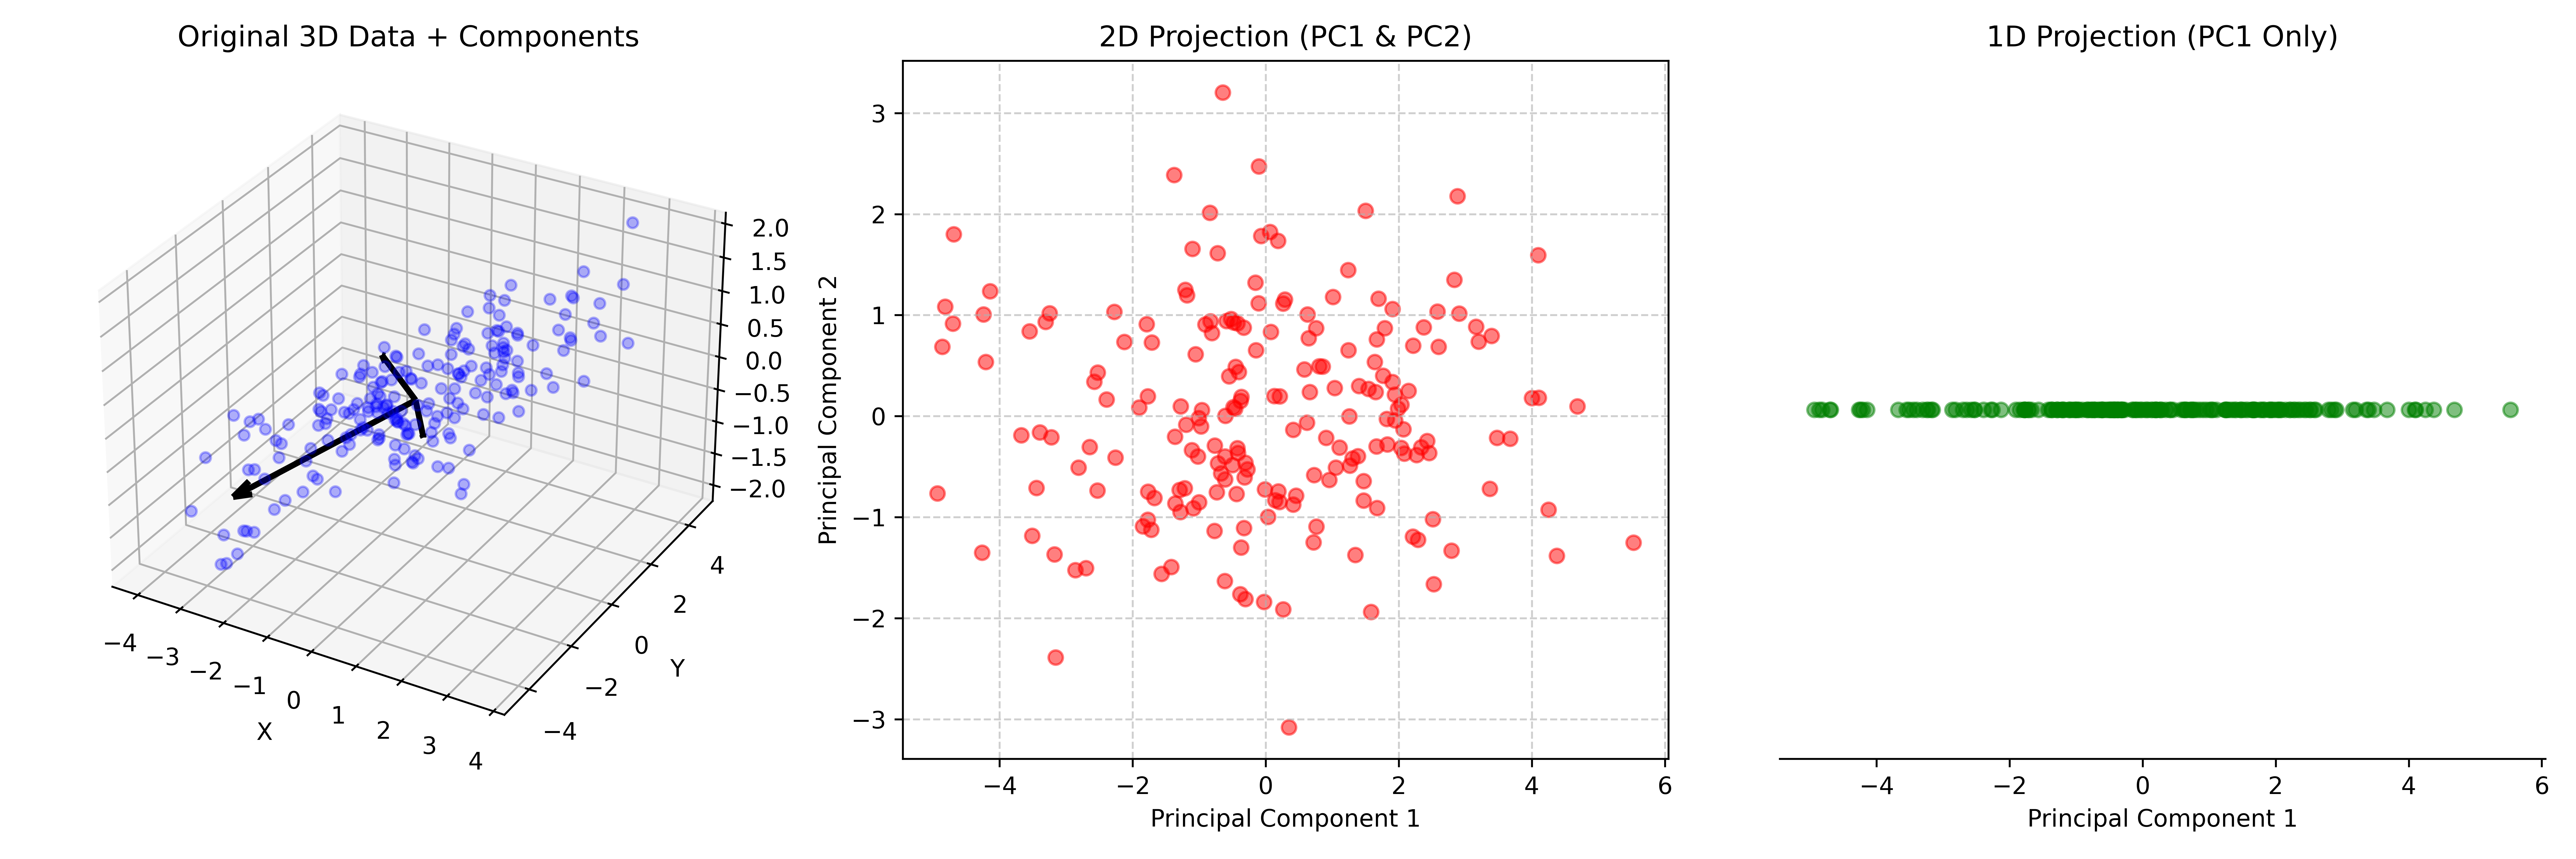
\includegraphics[width=\linewidth]{./img/pca_full_transformation}
		\end{figure}
	\end{frame}
	
\end{document}